For a quantum computer, multiple qubits are needed that are capable of interacting with each other. 
Thus, we need to make an array of the tweezers described in \cref{ch:tweezer}, spaced from each other in the order of micrometers. 
This can be done by sending several laser beams to the objective, each under slightly different angles. 
Experimentally, this could be realized using an \ac{AOD}: a device that diffracts light off of a sound wave in a crystal, where the degree of diffraction is controlled by a \ac{RF} signal. 
By using 2 AODs in an orthogonal configuration, each supplied by a superposition of RF signals, 2D Arrays have been successfully realized \cite{Manuel2016}. 
This principle is sketched in \cref{fig:CrossAOD}.

Nevertheless, one issue with this method is that there is little flexibility in varying the individual laser spot intensities because of the crossed configuration.
Therefore, \cite{Bergamini2004} showed a different method could be used to make tweezer arrays, making use of a \acf{SLM}, which was already briefly discussed in the previous chapter. 
With the SLM, it is in principle even possible to make 3D arrays of tweezers \cite{DiLeonardo2007,Barredo2016}, though we will limit ourselves to arrays in 2D in this work.

In \cref{sec:SLM} we will introduce the working principle and calibration of the SLM, as well as the algorithm used to compute the holograms. 
Next, in \cref{sec:SLMoperatoin} we elaborate how we used the SLM in the experiments and in \cref{sec:ArraysResults} we show the measured spot arrays.



\section{The Spatial Light Modulator}\label{sec:SLM}

A spatial light modulator is in essence a mirror that can imprint a computer generated hologram onto a beam of light, allowing the spatial shaping of this light.
Different types of SLMs can manipulate properties of light like amplitude, phase and polarization.
In this work a phase-only SLM was used, which as the name suggests can only control local phase of the incoming light field.
This is done by deploying a pixel array, where each pixel houses a liquid birifringent crystal.
By applying a voltage (electric field) over the pixel, the orientation of the liquid crystal molecules change, changing their effective refractive index.
This is shown in \cref{fig:LCoS}.

Because of crystals are birifringent they posses refractive indices among perpendicular axes, commonly referred to as the ordinary and extraordinary refractive indices respectively ($n_o$ and $n_e$). 
If the light travels a distance $t$ in a crystal unit of the SLM, the phase retardation will be $\phi_o = k t n_o$ and $\phi_e(V) = k t n_e(V)$ respectively (only the extraordinary axis can be modulated), such that the phase retarder can be represented by the Jones matrix \cite{Guzman2017}

\begin{equation}\label{eq:JonesMatrix}
    M = e^{i \phi_0} 
    \begin{pmatrix}
        e^{i(\phi_e-\phi_o)} & 0\\
        0 & 1
    \end{pmatrix}.
\end{equation}
Thus the phase retardance $\phi$ as a function of the applied voltage $V$ is \cite{Guzman2017}, using the birifringence parameter $\Delta n= n_e-n_o$

\begin{equation}\label{eq:ElectroOpticResponse}
    \phi(V) = k t(n_e(V) - n_0) t = \frac{2\pi}{\lambdaup}t \Delta n(V).
\end{equation}
To obtain voltage control over each individual pixel, the display is manufactured on a layer of silicon, making use of various semiconductor manufacturing technologies.
A sketch of the SLM pixels is shown in \cref{fig:LCoS}. 

As a result of diffraction from the various pixels, one can create arbitrary interference patterns in in the focal plane of a lens, which is sketched in \cref{fig:SLMLens}.
The use of SLMs has been extensively covered in our group by, for example \cite{Dijk2012,Bijnen2013,Bijnen2015}. 
Because the SLM used previously in our group suffered from amplitude modulation \cite{Dijk2012,Bijnen2015}, an unwanted effect, we purchased a newer model SLM. 
The model we use is the Meadowlark E-series 1920 x 1200 SLM.
Some key parameters of the SLM are presented in \cref{table:SLMspecs}.

\begin{table}[h]
    \centering
    \caption{Selection of specifications of the Meadowlark SLM.}
    \label{table:SLMspecs}
    \begin{tabular}{l | l}
        \textbf{Specification}          & \textbf{Value}        \\ \hline 
        Array size                      & 15.4 x 9.6 mm         \\ \hline
        Resolution                      & 1920 x 1080 pixels    \\ \hline
        Bit depth                       & 8 bit                 \\ \hline
        Diffraction efficiency          & 76-79\%   
    \end{tabular}
\end{table}

\begin{figure}
	\begin{subfigure}{.39\textwidth}
		\flushleft
		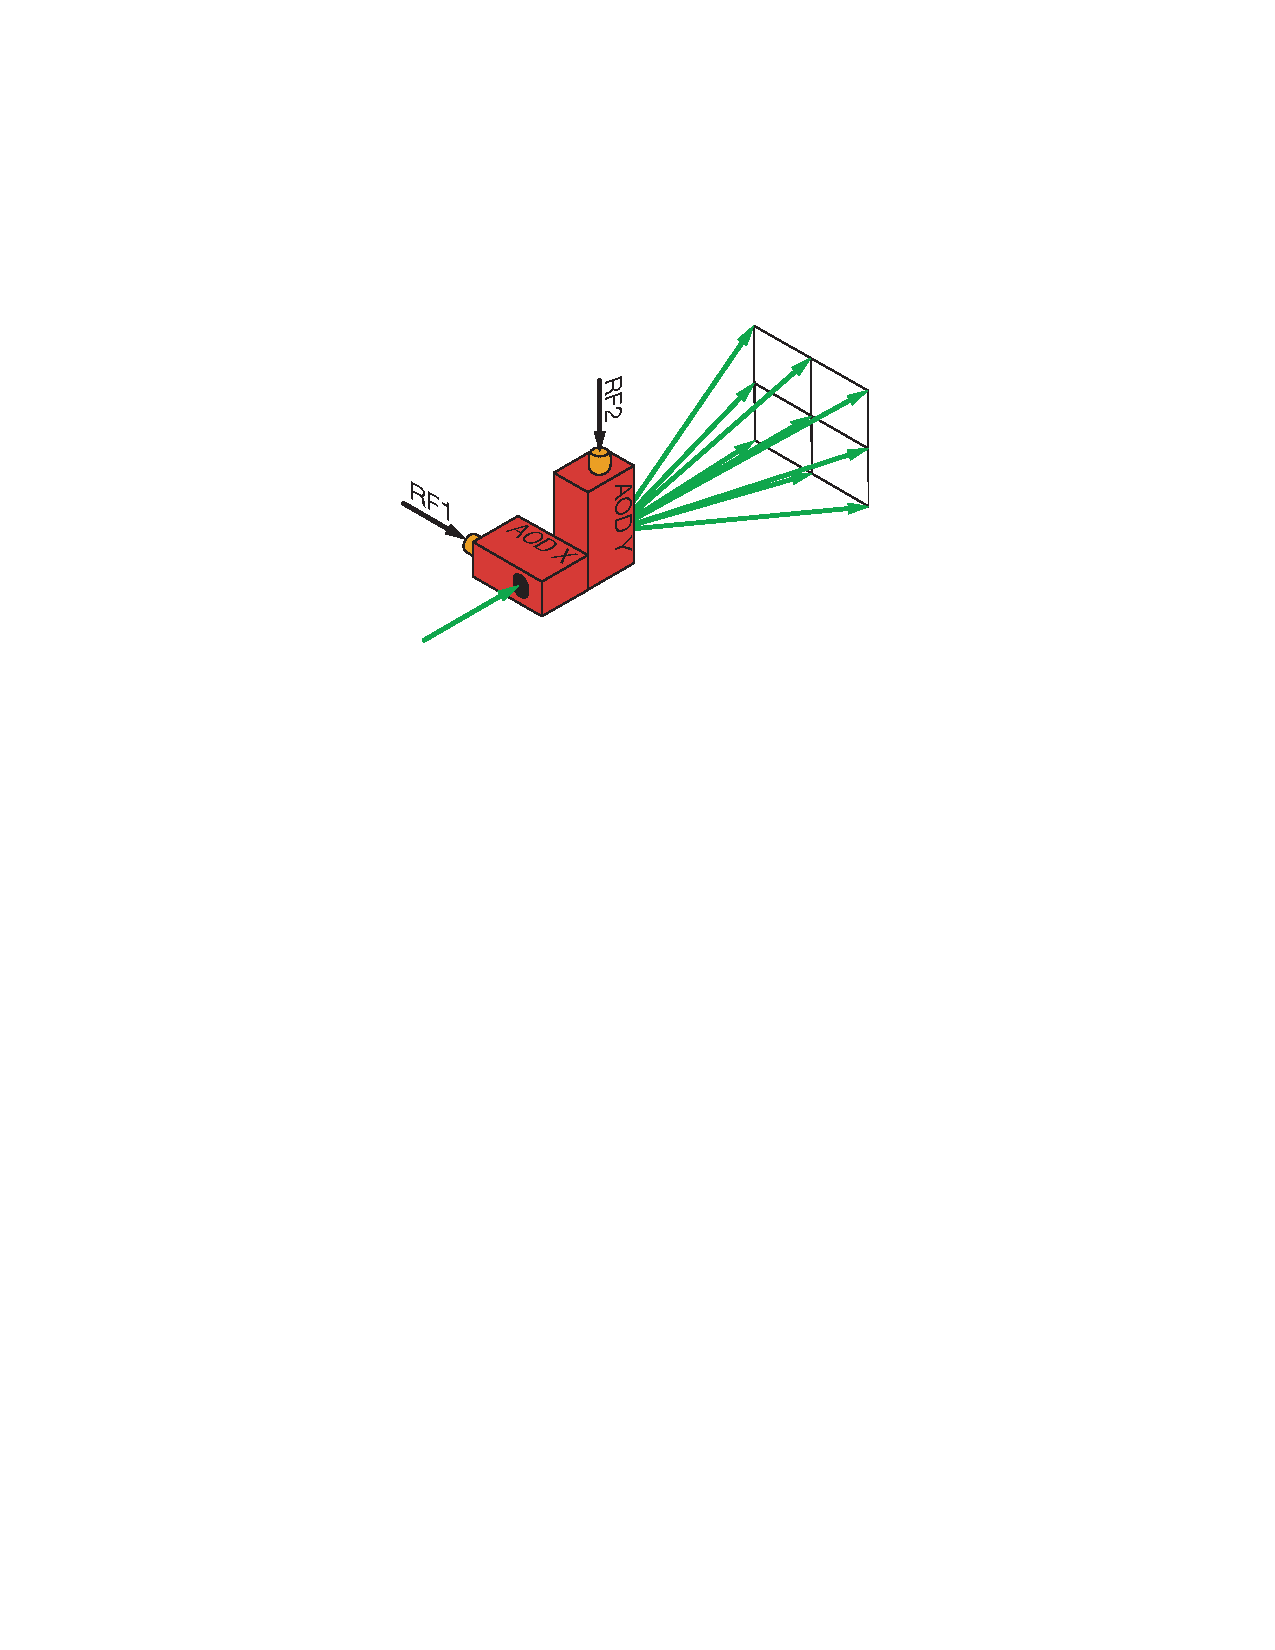
\includegraphics[height=4.25cm]{figures/crossAOD.pdf}
		\caption{}
		\label{fig:CrossAOD}
	\end{subfigure}
	\hfill
	\begin{subfigure}{.59\textwidth}
		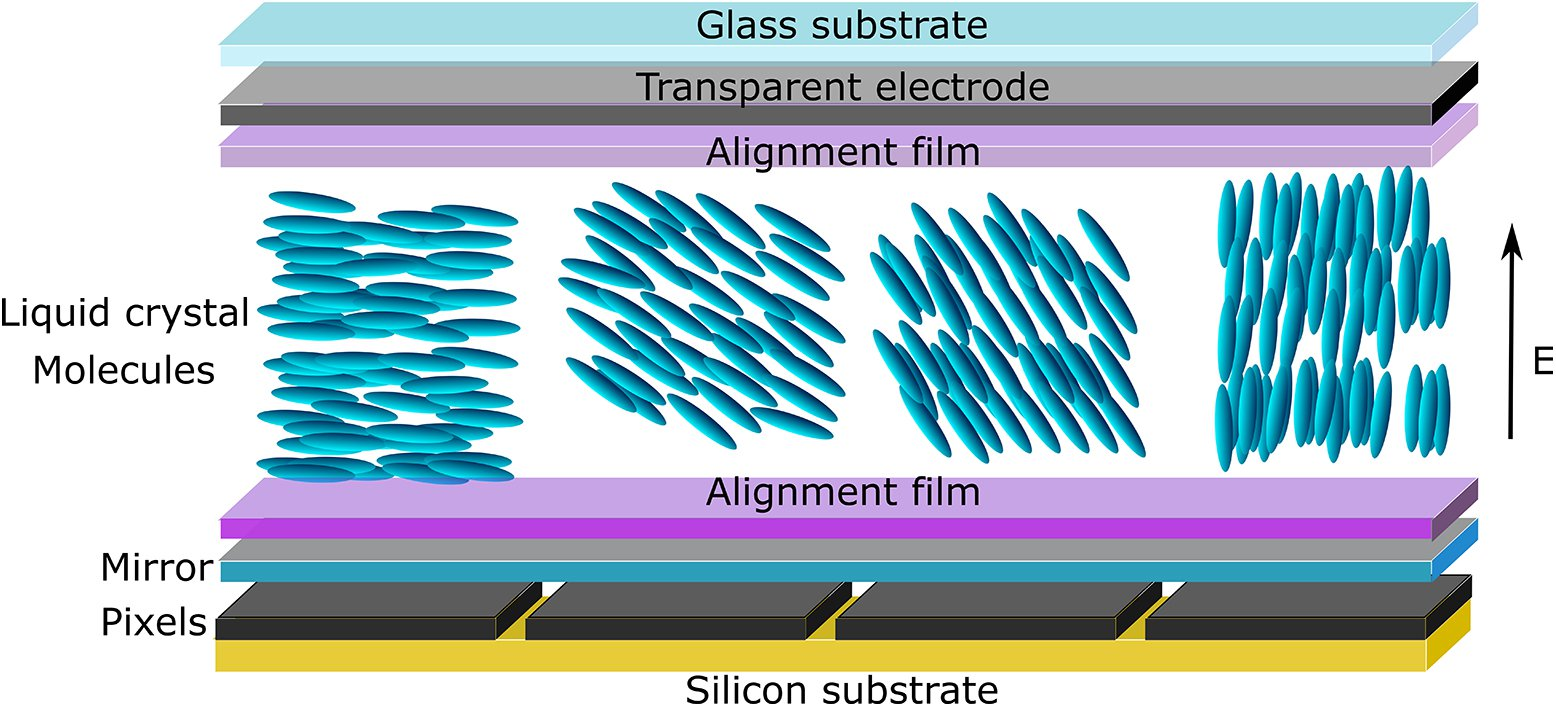
\includegraphics[height=4.25cm]{figures/LCoS.png}
		\caption{}
		\label{fig:LCoS}
	\end{subfigure}
	\caption{\textbf{a)} Two \ac{AOD}s in crossed configuration, used to make a 2D spot array. Figure from \cite{Cooper2018}. 
	\textbf{b)} The orientation of the liquid crystal cells changing as a function of the applied electric field \textit{E}. 
	Figure from \cite{Guzman2017}.}
\end{figure}

\subsection{Calibrating the Electro-Optic Response}

The refractive index $\Delta n(V)$ and therefore the light retardation $\phi(V)$ (\cref{eq:ElectroOpticResponse}) are not necessarily linear as a function of the applied voltage V. 
Thus it is needed to calibrate the electro-optic response of the \ac{SLM}, which equates to measuring the retardation $\phi$ as a function of the applied voltage $V$. 
This calibration serves two purposes:

\begin{enumerate}
    \itemsep=0pt
    
    \item Ensure the minimum to the maximum phase retardation corresponds to a $2\pi$ (one wave) phase retardation.
    
    \item Linearize the electro-optic response. 
\end{enumerate}
The calibration has to be performed because each individual SLM has a slightly different electro-optic response. 
Furthermore, it is wavelength specific, which is why we performed it for the wavelength relevant for Rb experiments at 820 nm. 
Measuring the electro-optic response directly is impossible because the light field oscillates with frequencies in the THz regime.
There are a variety of methods to measure it indirectly for a phase-only \ac{SLM}, however \cite{Li2019}.
We chose the diffractive calibration method, originally proposed by \cite{Zhang1994}.

The method works by imprinting a variety of Ronchi gratings onto the SLM, see \cref{fig:LUTCalibrationSetup}.
This is a pattern consisting of $M$ periods of width $w$ in the horizontal direction and a vertical height $H$ of alternating gray values $L_1$ and $L_2$.
A gray value is a 8 bit number representing the degree of modulation where 0 (white) mean no voltage while 255 (black) is maximum voltage. 
Assuming amplitude modulation between different gray levels is negligible (a fair assumption for phase-only SLMs), the electric field just after the SLM is proportional to the phase transmittance given by summing over the gratings $m$ \cite{Zhang1994}

\begin{equation}\label{eq:FieldAfterSLM}
    f(x',y') = \sum_{m=0}^{M-1} \left\{
    \operatorname{rect}\left(\frac{x'-m w - w/4}{w/2}\right) + e^{i \phi(L)} \operatorname{rect}\left(\frac{x'- m w - 3 w/4}{w/2}\right)
    \right\},
\end{equation}
where $\operatorname{rect}(\cdot)$ is the rectangular function. 
According to Fourier optics, if we place a lens after the SLM, the field in the \textit{Fourier} plane of the lens is the Fourier transform of the field after the SLM, as derived in \cref{eq:FraunhoferSimplified} as well as in \cref{eq:2Dcase}.
The intensity is thus for $y=0$ (we separate the different orders in the $x$-direction around $y=0$) the 2D Fourier transform $F = \mathcal{F}(f)$ \cite{Zhang1994}

\begin{equation}\label{eq:FourierIntensity}
    |F(p,0)|^2=
    \frac{M^2 w^2}{2}\operatorname{sinc}^2\left(\frac{M p w}{2}\right) \times
    \frac{1 + \cos{\left[\phi(L)+p w/2\right]}}{\cos^2(p w/4)}.
\end{equation}
In \cref{eq:FourierIntensity} $p=2\pi x/\lambdaup f$ is the Fourier transformed spatial coordinate. The intensity in the first order ($p=\pm 2\pi/w$) is

\begin{equation}\label{eq:IntensityFirstOrder}
    I_1(\phi) =
    \frac{8M^2w^2}{\pi^2} \left( 
    1-\cos{\phi(L)}
    \right),
\end{equation}
which we will use to fit the measurement data. Experimentally, we load a sequence of Ronchi gratings onto the SLM, looping $L_1$ from the minimum to the maximum gray value, while keeping $L_2$ constant. 
For our 8-bit SLM, this amounts to looping over 255 gray values.
For each hologram, separate the multiple diffraction orders using a $f=400$ mm lens (such that the spacing between the various orders is sufficient) and an aperture and record the power in the first order using a power meter.

The results are shown in \cref{fig:LUTcalibration}. 
Also shown is the result of fitting \cref{eq:IntensityFirstOrder}: the voltage response as a function of gray level. 
This fit was done with a software program provided by the manufacturer.
This is also called the gamma curve or \ac{LUT}.
The LUT is the 8-bit gray level to 10-bit voltage levels of the SLM, such that the electro-optic response is linear. 
As can be seen from \cref{fig:LUTcalibration}, the obtained LUT is rather non-linear, meaning the electro-optic response is also non-linear as expected.

\begin{figure}
	\begin{subfigure}{.54\linewidth}
	    \flushleft
		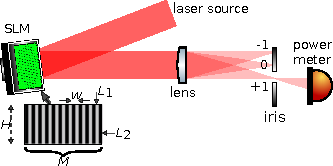
\includegraphics[height=4.2cm]{figures/LUTcalibrationSetup.pdf}
		\caption{}
		\label{fig:LUTCalibrationSetup}
	\end{subfigure}
	\hfill
	\begin{subfigure}{.44\linewidth}
	    \flushright
		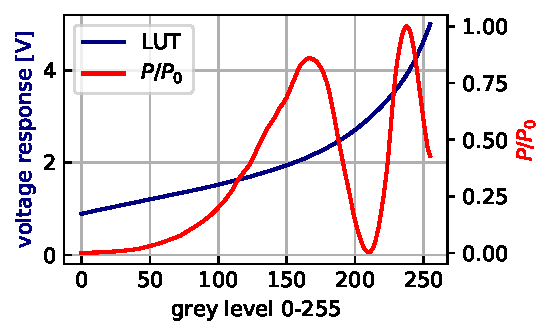
\includegraphics[height=4.2cm]{figures/LUTplot.pdf}
		\caption{}
		\label{fig:LUTcalibration}
	\end{subfigure}
	\caption{\textbf{a)} We put a Ronchi grating onto the SLM with gray values $L_1$ and $L_2$ We separate the diffraction orders using a $f=400$ mm lens and block all orders other than the $+1$ order using an iris. 
	\textbf{b)} Normalized power in the first order as a (\textcolor{red}{red}) and the fitted voltage response (\textcolor{blue}{blue}) as a function of the applied gray level $L_1 \in (0-255)$.}
\end{figure}


\subsection{Diffraction for Spot Arrays}\label{sec:PropagationDerivation}

With a linear voltage response established, it is time to look at how the formation of intensity patterns using a SLM works using the various pixels.
We will limit ourselves to producing diffraction patterns of spot arrays.
Labeling the pixels with $j$, the phase retardance is thus $\phi_j(x'_j,y'_j)$ where $(x',y')$ are Cartesian coordinates in the plane of the SLM.
Now, consider a laser with intensity distribution $|E_i(x',y')|^2$ hitting the SLM, it will pick up a phase factor such that after the SLM, the field is described as $E_i e^{i\phi(x',y')}$, as shown in \cref{fig:SLMLens}. 
The field will interfere with itself, until at infinity (or in the focal (Fourier) plane $z'=f$, $z=0$ of a lens) the distribution evolves to $|E_f(x,y,z)|^2$, where $(x,y,z)$ are Cartesian coordinates with the origin in the focus point of the lens as presented in \cref{fig:SLMLens}.

\begin{figure}
    \centering
    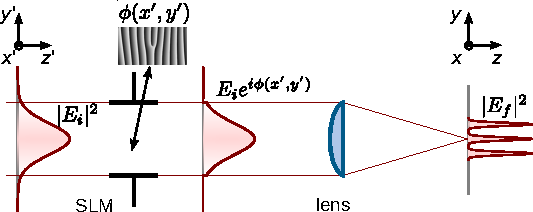
\includegraphics[width = 13cm]{figures/SLMfigure.pdf}
    \caption{Field with intensity distribution $|E_i|^2$ hitting the SLM, which due to its finite size acts as an aperture.
    The lens makes the resulting image $|E_f|^2$ in its focal plane.
    Also shown: two Cartesian coordinate systems in the SLM and focal plane. 
    Not to scale. 
    Adapted from \cite{Labuhn2016}.}
    \label{fig:SLMLens}
\end{figure}

The spots in the array will be labeled as $m$, which in general have coordinates $(x_m, y_m, z_m)$ in the Fourier plane, see \cref{fig:SLMgeometry}.
In reality, the distance between the SLM and the microscope objective is not the focal length $f$ of the objective, but this only adds a negligible phase factor \cite{Bijnen2013}.
As result of traveling from the pixel $j$ to the trap $m$, under paraxial approximation it can be derived the light field will experience a phase shift $\Delta_j^m$ \cite{DiLeonardo2007}

\begin{equation}\label{eq:PropagationPhase}
    \Delta_j^m = 
    \frac{2\pi z_m}{\lambdaup f^2} ({x'}_{j}^{2} + {y'}_{j}^{2}) 
    + \frac{2\pi}{\lambdaup f}(x'_j x_m + y'_j y_m).
\end{equation}
The SLM imprints a phase $\phi(x',y') = \phi_j$, leading to a complex SLM plane for pixel $j$ of

\begin{equation}\label{eq:SLMassumption}
    E_j(x',y') = E_j e^{i \phi_j}.
\end{equation}
Thus we can find the light field for trap $m$ by summing over $N$ pixels $j$ with contributions \cref{eq:PropagationPhase,eq:SLMassumption}.
In doing this, we assume uniform illumination of the SLM such that the amplitude is the same everywhere: $|E_i| = 1$.
A priori we know this assumption is not true: we illuminate the SLM with a Gaussian beam from an optical fiber.
However, as will become clear in a moment, the input intensity on the SLM will have no influence on the intensities in the focal plane and this assumption can be used without loss of generality.

In the focal plane, the complex light amplitude $V_m$ (for this section, we will denote the complex light field in the Fourier plane as $V$ similar to \cite{DiLeonardo2007}) for trap $m$ can be found by summing over all pixels and using a discrete version of the Fresnel diffraction integral \cite{Leseleuc2018}

\begin{equation}\label{eq:DiffractionFormula}
    V_m = e^{i k \left(2 f + z_m\right)}
    \frac{d^2}{i \lambdaup f} \sum_{j=1}^N e^{i(\phi_j - \Delta_j^m)},
\end{equation}
where $d$ is the pixel pitch of the SLM. 
But we are really only interested in the intensity $I_m =|V|^2$ of each spot, not the phase.
Omitting the pre-factors in \cref{eq:DiffractionFormula} thus yields

\begin{equation}\label{eq:Vm}
    V_m \propto \sum_{j} e^{i(\phi_j - \Delta_j^m)}.
\end{equation}
So the contribution for trap $m$ really arises from all pixels $j$. 
As a result, the spatial profile of the input field does not matter, which is an advantage of this type of algorithm. While \cref{eq:Vm} can be used to construct 3D geometries, an instructive example is setting $z=0$ first \cite{DiLeonardo2007}, for which the quadratic term of \cref{eq:PropagationPhase} vanish.
The result should be a 2D array of amplitudes

\begin{equation}\label{eq:2Dcase}
    V_m \propto \sum_j e^{i\phi_j} \exp{\left(
    - i 2\pi \left[
    \frac{x_m}{\lambdaup f} x_j + \frac{y_m}{\lambdaup f} y_j
    \right]
    \right)},
\end{equation}
Wwich is the 2D \ac{DFT} of $e^{i\phi}$ evaluated at spatial frequencies $x_m/\lambdaup f$ and $y_m/\lambdaup f$ in $x$ and $y$ respectively \cite{DiLeonardo2007,Bijnen2015}, similar to \cref{eq:FraunhoferSimplified}.
This has the DFT is much faster to evaluate than the general case of the diffraction formula \cref{eq:Vm} using the \ac{FFT}.
In this work, we only use 2D arrays and could in principle use \cref{eq:2Dcase} to speed up calculations.
Because we only have to compute a couple of holograms, we simply used \cref{eq:Vm}.

\subsection{Computing the Hologram}\label{sec:GSW}

\Cref{eq:Vm} gives the amplitudes of an array of spots given an array of phases $\phi_j$, but we are interested in the reverse problem: what is the hologram $\phi_j$ to be applied, such that we get the spot intensities $|V_m|^2$? 
Because the equations describing light propagation are time-symmetric, this phase will be the result of $M$ coherent light sources radiating with $w_m e^{i \theta_m}$, picking up a propagation phase described by \cref{eq:PropagationPhase}, leading to a complex amplitude in the \ac{SLM} plane of \cite{DiLeonardo2007,Leseleuc2018}

\begin{equation}\label{eq:InterferencePattern}
    E_j (x',y') = \sum_m w_m \exp{
    i\left(\Delta_j^m + \theta_j\right)
    }.
\end{equation}
But producing the the light field in \cref{eq:InterferencePattern} requires doing phase as well as amplitude modulation, which is not possible: the SLM can only do phase modulation.
So in this step in the algorithm, we take the argument of  \cref{eq:InterferencePattern} yielding the following hologram

\begin{equation}\label{eq:Argument}
    \phi_j = \text{arg}\left\{
     \sum_m w_m \exp{
    i\left(\Delta_j^m + \theta_j\right)
    }
    \right\}.
\end{equation}
But because the amplitude modulation is lost, this will not be the correct hologram.
The solution to this problem was solved by \cite{Gerschberg1972}, who pioneered the \ac{IFTA} algorithm or Gerschberg-Saxton algorithm.
The core idea of the algorithm is to virtually propagate light between SLM and focal planes, updating the hologram in the SLM plane and  intensities in the Fourier plane in an iterative fashion, until the solution converges to the desired values.
For a more detailed description of an implementation of IFTA algorithms the reader is referred to \cite{Bijnen2013,Bijnen2015}.

For 3D spot arrays, (inverse) Fourier transforms cannot be used, and the algorithm was extended using \cref{eq:Vm,eq:Argument} by \cite{DiLeonardo2007}. 
This algorithm is called the \ac{GSW} algorithm, which is sketched in \cref{fig:GSWalgorithm}.

\subsubsection*{The Algorithm}

\begin{itemize}
    \item Starting with hologram $\phi_j^k$ we use the diffraction equation \cref{eq:Vm} to compute the complex amplitudes of the spot array $V_m^{k+1}$. 
    
    \item From the amplitudes, we find new weight factors $w_m^k$ and phases $\theta_m^k$, which are used to compute a new hologram using the interference equation \cref{eq:Argument}.
    
    \item Then, the iteration counter $k$ is increased, the hologram is updated and the procedure repeats. 
\end{itemize}
As a starting point for a hologram, $\phi_j^{k=0}$ is computed by using \cref{eq:Argument} for an array of traps of uniform intensities $w_m^{k=0} = 1$ and random phases $\theta_m^{k=0}$.
After each iteration, the diffraction efficiency $e$ (the real part of the complex interference pattern) and the uniformity $u$ of the array $V_m$ should increase until convergence, yielding a set of target amplitudes $V_m$ as well as a hologram $\phi_j$ that produces this set of amplitudes.
The definitions of $\{e,u\}$ are 

\begin{equation}\label{eq:EfficiencyUniformity}
    e = \frac{1}{M}\sum_m I_m = \frac{1}{M}\sum_m |V_m|^2, 
    \quad 
    u = 1-\frac{\text{max}(I_m)-\text{min}(I_m)}{\text{max}(I_m)+\text{min}(I_m)},
\end{equation}
which are evaluated in the algorithm after each iteration $k$. 
The algorithm was implemented in Python by Ivo Knottnerus as part of his PhD research.
Because the SLM has $\sim 2$ million pixels, converting to and from the SLM plane, so performing equations \cref{eq:Vm,eq:Argument} can be time consuming depending on the desired pattern.
Therefore, these computations are performed on a graphics card using the \textit{PyOpenCL} library. 
After a couple tens of iteration steps, we typically see the diffraction efficiency convergence to $e \sim 0.93$ and the theoretical target uniformity to $u \sim 0.999$.

\begin{figure}
\centering
	\begin{subfigure}{.56\textwidth}
		\centering
		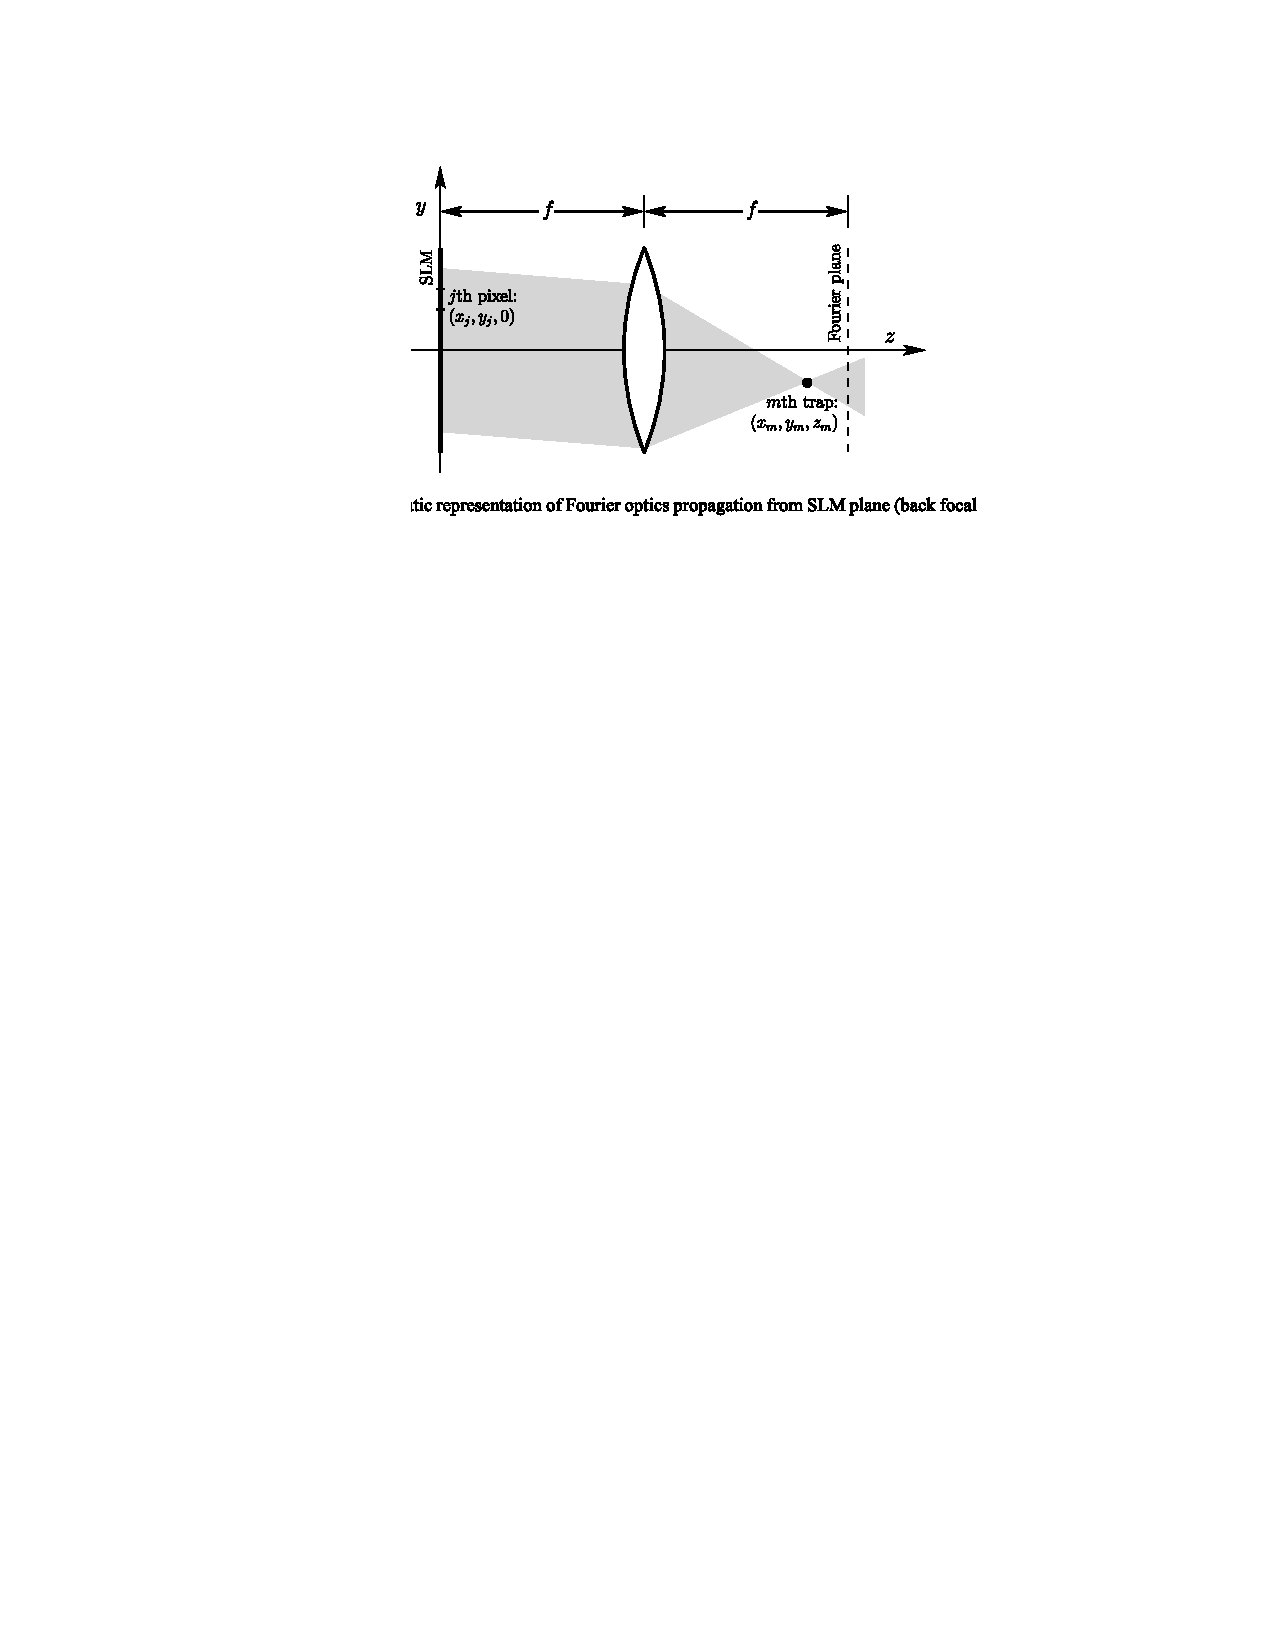
\includegraphics[height=5cm]{figures/SLMgeometry.pdf}
		\caption{}
		\label{fig:SLMgeometry}
	\end{subfigure}
	\begin{subfigure}{.43\textwidth}
		\centering
		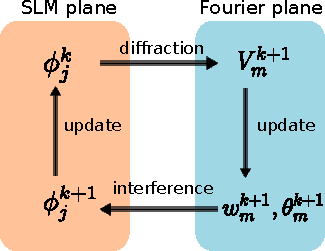
\includegraphics[height=5cm]{figures/WeightedGerschbergSaxton.pdf}
		\caption{}
		\label{fig:GSWalgorithm}
	\end{subfigure}
	\caption{\textbf{a)} SLM plane with phases $\phi_j(x,',y',z=0)$ for pixel $j$, as well as the focal plane or Fourier plane with trap coordinates for trap $m$ of $(x_m,y_m,z_m)$. 
	Figure from \cite{DiLeonardo2007}. 
	\textbf{b)} The \ac{GSW} algorithm visualized.
	The light field is virtually propagated between the SLM and focal planes using \cref{eq:Vm,eq:Argument}, continuously updating the weight factors $w_m^k$ as well as the hologram $\phi_m^k$.}
	\label{fig:GerschbergSaxton}
\end{figure}


\section{Operating the SLM}\label{sec:SLMoperatoin}

A typical hologram from the algorithm discussed in the previous section is shown in \cref{fig:Array}.
But to implement the SLM in our optical tweezer experiment, this is not the only pattern we apply onto the SLM.
The other contributions are discussed below and added onto the hologram as well.
In the end, the modulo $2\pi$ of the total pattern is computed (retarding a wave by $2\pi$ is the same as doing nothing of course).


\begin{figure}
	\begin{subfigure}{.18\linewidth}
		\centering
		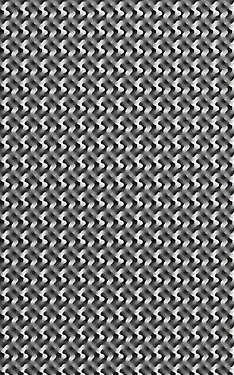
\includegraphics[height=4cm]{figures/SLMphase/array.jpg}
		\caption{}
		\label{fig:Array}
	\end{subfigure}
	%
	\begin{subfigure}{.18\linewidth}
		\centering
		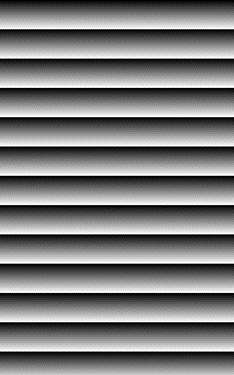
\includegraphics[height=4cm]{figures/SLMphase/linear.jpg}
		\caption{}
		\label{fig:Linear}
	\end{subfigure}
	%
	\begin{subfigure}{.18\linewidth}
		\centering
		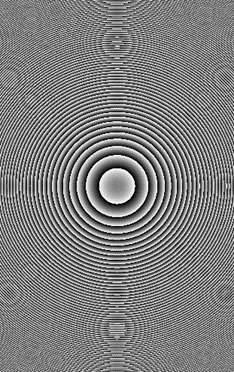
\includegraphics[height=4cm]{figures/SLMphase/lens.jpg}
		\caption{}
		\label{fig:Lens}
	\end{subfigure}	
	%
	\begin{subfigure}{.18\linewidth}
		\centering
		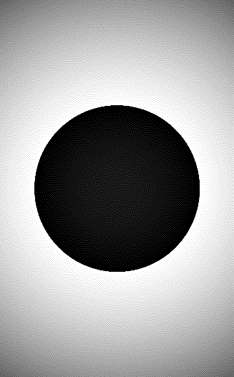
\includegraphics[height=4cm]{figures/SLMphase/flatness.jpg}
		\caption{}
		\label{fig:Flatness}
	\end{subfigure}
	%
	\begin{subfigure}{.18\linewidth}
		\centering
		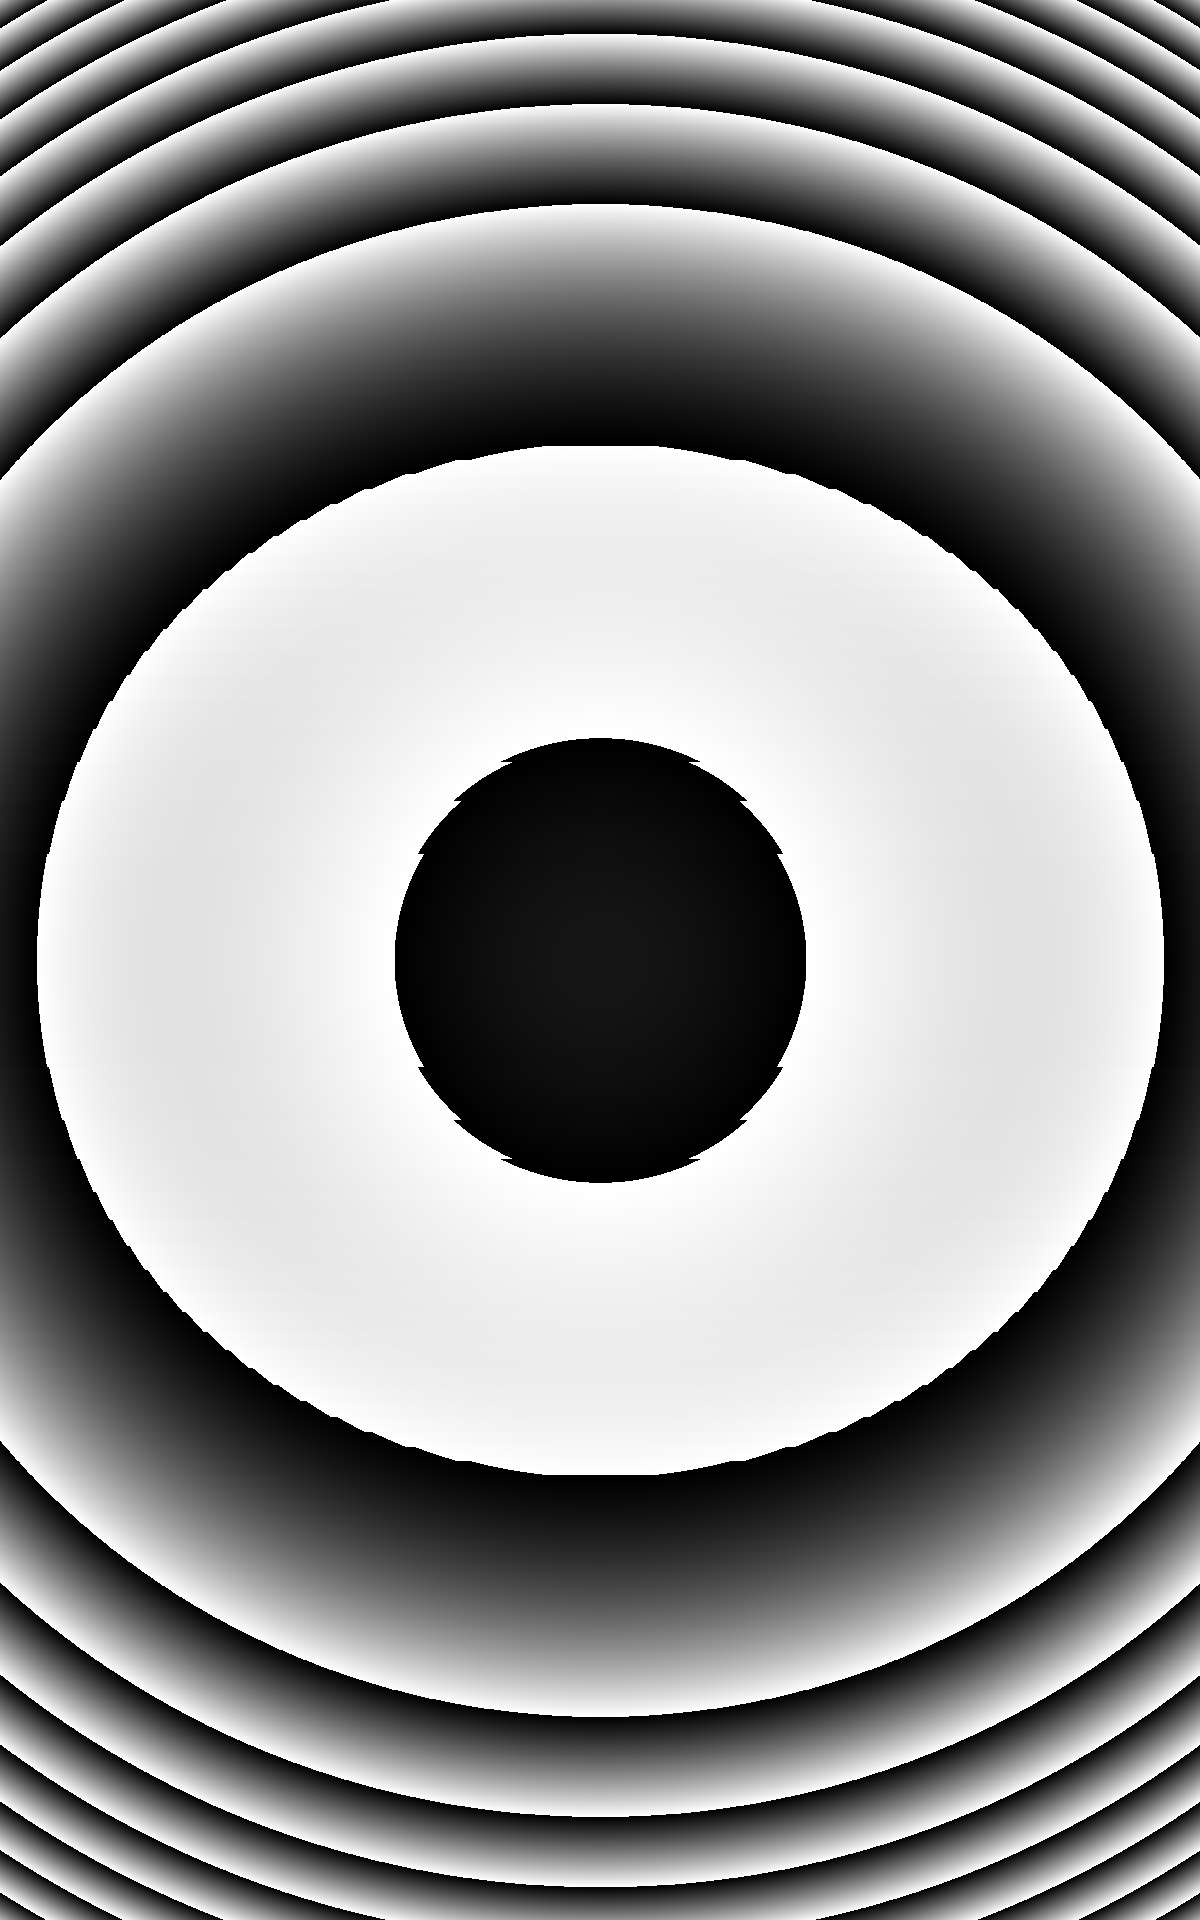
\includegraphics[height=4cm]{figures/SLMphase/zernike.jpg}
		\caption{}
		\label{fig:Zernike}
	\end{subfigure}
	%
	\begin{subfigure}{0.055\linewidth}
	    \centering
	    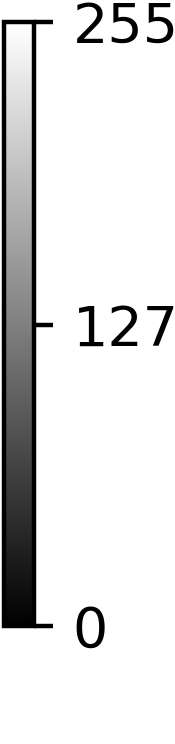
\includegraphics[height = 3.5cm]{figures/SLMphase/colorbar.jpg}
	\end{subfigure}
	%
	\caption{
	\textbf{a)} Hologram obtained from the \ac{GSW} algorithm.
	\textbf{b)} Blazed grating, used to move the diffraction pattern away from the optical axis. Zoomed in for the sake of visibility.
	\textbf{c)} Lens phase applied to use the SLM as the first lens of a telescope with magnification $0.42$.
	\textbf{d)} Optical flatness correction pattern as provided by the manufacturer.
	\textbf{e)} Aberration correction phase applied onto the SLM.
	}
	\label{fig:SLMphase}
\end{figure}


\subsection{Diffraction Orders}\label{subsec:Diffraction}

Because the SLM has individual pixels with constant pitch $d$, the device acts effectively as a diffraction grating, so will be reflected in a variety of orders. 
It is well known from diffraction theory that in both $x$ and $y$ these diffraction angels $\theta_l$ of order $l$ occur at \cite{Hecht2002}

\begin{equation}
    \theta_l = \arcsin\left(\sin\theta_i - l\frac{ \lambdaup}{d}\right)
\end{equation}
for incident angle $\theta_i$. 
The $l=0$ order contains the most power and is the only order that is used, the other orders are blocked using an aperture. 
But apart from higher diffraction orders, there will always be a fraction of light that is not modulated. 
For example, there is a tiny amount of unused space between and around the pixels.
This unmodulated light is separated from the modulated light by imposing a linear phase on top of the pattern (tilt phase) which translate the desired pattern away from the undiffracted light.
Subsequently the undiffracted light is blocked in an intermediate focus point using an iris, which is also used to block higher diffraction orders.
The type of linear phase used is shown in \cref{fig:Linear}.
Because the phase retardance is capped at $2\pi$, a saw-tooth-like pattern emerges.
In reality, we use a period of just 8 pixels, so for better visibility we only show a tiny part of the grating in the figure.

\subsection{Finite Aperture Size}\label{subsec:ApertureSize}

In order to employ the maximum amount of degrees of freedom the SLM has to offer, and therefore the maximum drawing area in the focal plane of the Fourier lens, all of the pixels should be illuminated. 
However, because the incident beam is described by a Gaussian, this will lead to power loss as a result of light not falling on the active pixel area. 
The ideal incident waist size is thus a compromise between power efficiency on the one and amount of pixels used on the other side.
    
We can estimate this power loss by shining a Gaussian beam $G(x,y)$ of width $w(z)$ and power $P_0$ onto a rectangular aperture of dimensions $(2S_x, 2S_y)$ where $S_{x,y}$ are the semi-widths of the aperture. 
The relative power transmission $P/P_0$ can be found by integrating the intensity of the beam \cref{eq:GaussianBeamIntensity} in Cartesian coordinates over the aperture

\begin{equation}\label{eq:RectAperturePower}
    \frac{P}{P_0} =
    \iint G(x,y) dA=
    \text{erf}\left(\frac{\sqrt{2}S_x}{w(z)}\right) \text{erf}\left(\frac{\sqrt{2}S_y}{w(z)}\right)
\end{equation}
where erf($\cdot$) denotes the error function. 
The optimum incident beam size $w(z)$ is thus a compromise between drawing area and power efficiency. 
We have decided to use $w(z) = 4.8$ mm, which is about the size of the short axis $S_x = 4.9$ mm, such that we illuminate the entire \ac{SLM} and the power transmission as a result of the finite rectangular aperture is $\sim 95$\%.

\subsection{Demagnification}

The $w = 4.8$ mm beam needs to be adapted to the $R = 2$ mm radius of the microscope objective, in order to not lose almost all of the power. 
As discussed in \cref{ch:tweezer}, we use a 2 mm waist at the microscope objective, so the magnification should be $M = 2.0 / 4.8 \sim 0.42$. 
We do this by applying a lens phase onto the SLM shown in \cref{fig:Lens}. 
Finally, \cref{fig:Zernike} shows the Zernike correction pattern as found in \cref{ch:tweezer}.

\subsection{Optical Flatness}\label{subsec:Flatness}

Because of manufacturing imperfections, the SLM chip will not be perfectly flat on the scale of light wavelengths. 
This error is different for invididual SLM units.
The flatness of our chip was measured by manufacterer Meadowlark to have a RMS flatness of $\sim 0.18\lambdaup$.
The shape of the flatness was measured as well, so we can correct for the error by subtracting this phase pattern. 
The correction used is shown in \cref{fig:Flatness}.

\subsection{Aberration Correction}\label{subsec:AberrationCorrection}


We can look at the effect of this material using the sketch in \cref{fig:SphericalSketch}. 
For paraxial rays, ($\alpha_0 \rightarrow 0$), \cref{eq:SphericalFocus} reduces to $d(1-n_r)$. 
Subtracting this from \cref{eq:SphericalFocus} and Taylor expanding up to fourth order in $\alpha_0$ yields 

\begin{equation}\label{eq:FocusDifference}
    \delta f_{\text{marginal}} - \delta f_{\text{paraxial}} \approx
    \frac{d \tan^2{\alpha_0}}{2n} (1-n_r^2) - \frac{3d \tan^4{\alpha_0}}{8n}(1-n_r^2)^2+\mathcal{O}(\tan\alpha_0^6).
\end{equation}
Multiplying \cref{eq:FocusDifference} with $2\pi(n-n_0)/\lambdaup$ and converting to a radial dependence as $\tan{\alpha_0}= \text{NA} \times r/R$ yields \cite{Iwaniuk2011}

\begin{equation}\label{eq:ConversionRadial}
    \phi(r) \approx \frac{\pi d}{\lambdaup}(1-n_r)\left[
    \left(\text{NA}\frac{r}{R}\right)^2(1-n_r^2)-\frac{3}{4}\left(\text{NA}\frac{r}{ R}\right)^4(1-n_r^2)^2
    \right].
\end{equation}
This is a function that can be decomposed in Zernike polynomials.
The Zernike polynomials are a set of orthogonal polynomials on the unit disk, related to optical aberrations. 
The coordinates on the unit disk can be denoted as $\rho = r/R$ and $\theta \in (0, 2\pi)$, such that the wavefront $\phi(\rho,\theta)$ can be expanded in terms $R_n^m(\rho)\cos{m\theta}$ and $R_n^m\sin{m\theta}$ where 

\begin{equation}\label{eq:ZernikeRadial}
    R_{n}^{m}(\rho)=
    \sum_{s=0}^{(n-m) / 2}
    \frac{(-1)^{s}(n-s) !}{s !\left((n+m)/2-s\right) !\left((n-m)/2-s\right) !} \rho^{n-2 s}
\end{equation}
is the radial Zernike polynomial set \cite{Mahajan94}. But it turns out \cref{eq:ConversionRadial} only has to nonzero $R_n^m$ terms: $R_2^2 = \rho^2$, which is a defocus aberration and $R_4^4 =\rho^4$ which is a third order spherical aberration. It is not needed to correct the defocus, leaving only the $\rho^4$ contribution, which is shown in \cref{fig:AberrationTerm}.

\begin{figure}
    \centering
    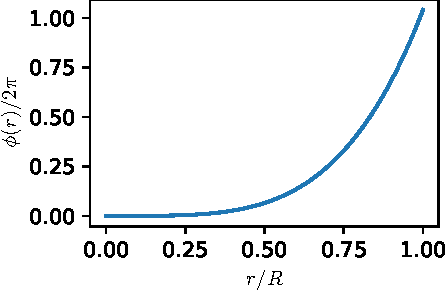
\includegraphics[width=0.4\textwidth]{figures/SphericalAberrationTerm.pdf}
    \caption{Phase correction applied onto the SLM to correct the third order spherical aberration as a function of the normalized radial coordinate $\rho=r/R$.}
    \label{fig:AberrationTerm}
\end{figure}




\section{Arrays of tweezers}\label{sec:ArraysResults}

Using holography and the SLM, we can make arbitrary arrays of spot using the algorithm discussed in \cref{sec:GSW}. 
We limited ourself to arrays of $n \times n \times 1$ pixels in the $x$, $y$ and $z$-directions respectively, where $n \in (1,2\ldots10)$. 
Phase masks were made using the algorithm implemented by Ivo Knottnerus running it for several hundred iterations, to get uniformities $>0.9999$ (In the \ac{GSW} algorithm, uniformities will get arbitrarily high for more iterations). 
In we show a result, where we plot the calculated diffraction pattern in the focal plane. The theoretical diffraction efficiency: the real part of the interference in the focal plane from the light propagation equation was found to be on the order of $e \sim 0.92$ (\cref{eq:EfficiencyUniformity}, irrespective of the amount of spots made, similar to the original publication of this algorithm \cite{DiLeonardo2007}.
In ... we show the theoretical diffraction result as found by the program, the computed hologram, as well as the measured pattern from the camera. 

\begin{mdframed}
    \subsection*{About the Units in the Fourier Plane}
    
    It is not nesessary necessary for the algorithm to take the exact optical setup into account.
    For the purposes of producing phase masks, we discard the telescope and treat the microscope objective as an ideal lens with focal length $f = 4$ mm, as also shown in \cref{fig:SLMgeometry}.
    In this case, smallest feature that can be produced in the Fourier plane is the diffraction-limited spot from the size of the SLM dimenions which can be considered a rectangualar aperture \cite{Bijnen2013,Bijnen2015}:
    
    \begin{equation}\label{eq:FocalUnit}
        \Delta x \times \Delta y = \frac{2\lambdaup f}{S_x} \times \frac{2 \lambdaup f}{S_y}
    \end{equation}
    \cref{eq:FocalUnit} are known as focal units and they are a natural unit to use in the Fourier plane.
    However, this will not fully apply to us, because we conjugate the short axis of the SLM to the aperture radius of the lens (objective), such that the extra pixels in the long axis of the SLM are effectively not used. 
    Therefore, we can set $S_x = S_y$ and the focal units will be the same in $x$ and $y$.
\end{mdframed}
    



\subsection{Spot Detection}

We make an arbitrarily sized array of optical tweezers. For detecting maxima locations, we could simply set pixels above a certain count threshold as a maxima. The disadvantage of this is that a noisy pixel could be detected as a spot, which would hinder analysis. 

To combat this, we first convolute the image with a Laplacian of Gaussian filter, which first smoothes the image to reduce noise. Subsequently it computes the 2D laplacian to detect edges. If this second derivative is above a certain threshold, we detect the edge as a spot. If the detected amount of spots is not the expected amount, we can easily tune the threshold. The camera image is cropped into regions of interest around the spots marked by the Laplacian of Gaussian filter. 

\subsection{Spot Fitting}

We fitted the tweezer arrays using the same Gaussian used in the previous chapter (\cref{eq:2DGaussian}, with for each spot, numbered $k$, 5 fit parameters: the amplitude ('trap depth') $U_0$, the peak center $(x_0, y_0)$ as well as the sigmas in both cartesian coordinates $\sigma_x$ and $\sigma_y$:

\begin{equation}\label{eq:2DGaussianNumberK}
    U_k(x,y) = U_{0,k}\exp{\left(\frac{-(x_k-x_{0,k})^2}{2\sigma_{x,k}^2}\right)}
    \exp{\left( \frac{-(y_k-y_{k,0})^2}{2\sigma_{k,y}^2} \right)}
\end{equation}

So in principle we allow non circular spots, but we extract the waist $w_k$ of each spot as $w_k = \sigma_{x,k} + \sigma_{y,k}$